\documentclass[11pt]{article}

\usepackage{fancybox}


\usepackage{color}
\usepackage{url}
\usepackage[margin=1in]{geometry}
\usepackage{setspace}
\usepackage{lscape}
\usepackage{afterpage}

\setlength{\parskip}{1em}%
\setlength\parindent{0pt}
\renewcommand{\textfraction}{0.0}
\renewcommand{\topfraction}{1.0}
%\renewcommand{\textfloatsep}{5mm}

\usepackage{comment}
% Definitions of handy macros can go here
\usepackage{amsmath,amssymb,amsthm,bm,mathtools}
\usepackage{multirow}
\usepackage{extarrows}
\usepackage{dsfont,multirow,hyperref,setspace,natbib,enumerate}
%\usepackage{dsfont,multirow,hyperref,setspace,enumerate}
\hypersetup{colorlinks,linkcolor={blue},citecolor={blue},urlcolor={red}} 
\usepackage{algpseudocode,algorithm}
\algnewcommand\algorithmicinput{\textbf{Input:}}
\algnewcommand\algorithmicoutput{\textbf{Output:}}
\algnewcommand\INPUT{\item[\algorithmicinput]}
\algnewcommand\OUTPUT{\item[\algorithmicoutput]}

\mathtoolsset{showonlyrefs=true}



\theoremstyle{plain}
\newtheorem{thm}{Theorem}[section]
\newtheorem{lem}{Lemma}
\newtheorem{prop}{Proposition}
\newtheorem{pro}{Property}
\newtheorem{assumption}{Assumption}

\theoremstyle{definition}
\newtheorem{defn}{Definition}
\newtheorem{cor}{Corollary}
\newtheorem{example}{Example}
\newtheorem{rmk}{Remark}


\setcounter{figure}{0}   
\setcounter{table}{0}  



\newcommand{\of}[1]{\left(#1\right)}
\newcommand{\off}[1]{\left[#1\right]}
\newcommand{\offf}[1]{\left\{#1\right\}}
\newcommand{\aabs}[1]{\left|#1\right|}



%\usepackage{xcolor}

\newcommand{\cmt}[1]{{\leavevmode\color{red}{#1}}}


\usepackage{dsfont}
\usepackage{multirow}

\DeclareMathOperator*{\minimize}{minimize}


\usepackage{mathtools}
\mathtoolsset{showonlyrefs}
\newcommand*{\KeepStyleUnderBrace}[1]{%f
  \mathop{%
    \mathchoice
    {\underbrace{\displaystyle#1}}%
    {\underbrace{\textstyle#1}}%
    {\underbrace{\scriptstyle#1}}%
    {\underbrace{\scriptscriptstyle#1}}%
  }\limits
}

% adjust table separation
%\setlength{\tabcolsep}{6pt} % Default value: 6pt
%\renewcommand{\arraystretch}{1.5}

\def\fixme#1#2{\textbf{\color{red}[FIXME (#1): #2]}}

\usepackage{xr}
\makeatletter
\newcommand*{\addFileDependency}[1]{% argument=file name and extension
  \typeout{(#1)}
  \@addtofilelist{#1}
  \IfFileExists{#1}{}{\typeout{No file #1.}}
}
\makeatother
\newcommand*{\myexternaldocument}[1]{%
    \externaldocument{#1}%
    \addFileDependency{#1.tex}%
    \addFileDependency{#1.aux}%
}
\myexternaldocument{jcgs-tensor}
\myexternaldocument{supp}


\input macros.tex

\usepackage[english]{babel}
\usepackage[dvipsnames]{xcolor}

\usepackage{enumitem,kantlipsum}

\title{\textbf{Response Letter}}

\date{}
\author{}


%\setstretch{1.125}
\begin{document}

\maketitle
\vspace{-1.5cm}

We are grateful to the reviewers for their careful reading and thoughtful comments. Please note that the \textbf{Response to Major Comments Summarized by Editor} consists of general comments raised by both reviewers. We address these issues upfront {\bf in pages 1-7 of this letter}. 

\begin{center}
    \textbf{Response to Major Comments Summarized by Editor}
\end{center}

\begin{enumerate}[wide, labelwidth=!, labelindent=0pt]
    \item \textit{Comparison with other related methods should be included as pointed out by a reviewer.}
    
    \textbf{Response:} We thank the editor and both reviewers for pointing out additional related literature. Some references \citep{chi2012tensors, hong2020generalized, raskutti2019convex} were already included in the first version, but we have added more comparisons in the revision. We have also added other relevant papers suggested by reviewers. The current comparison consists of 12 tensor regression/factorization methods. Moreover, we have revised our numerical experiments substantially to compare our method with more recent work. Specifically, 
    \begin{enumerate}[wide, labelwidth=!, labelindent=0pt]
        \item we have added discussions about unsupervised model in Section~\ref{sec:intro}: 
        \begin{quote}
            ``...The first line is a class of \textit{unsupervised} tensor decomposition such as classical Tucker and CP decomposition~\citep{de2000multilinear, kolda2009tensor, wang2017tensor} and generalized decomposition for non-Gaussian data \citep{chi2012tensors, tarzanagh2019regularized,hong2020generalized,  li2020generalized}. Regardless of the implementation, the unsupervised methods aim to find the best low-rank representation of a data tensor alone. In contrast, our model is a \textit{supervised} tensor learning, which aims to identify the association between a data tensor and multiple features. The low-rank factorization is determined jointly by the tensor data and feature matrices in our model."
        \end{quote}
        
        \item we have added discussions about tensor-on-tensor models in Section~\ref{sec:intro}: 
        \begin{quote}
            ``...The second line of work studies the tensor-to-tensor regression. This category is further divided into three scenarios, depending on whether tensor is treated as predictors~\citep{zhou2013tensor,raskutti2019convex,han2020optimal}, as responses~\citep{li2017parsimonious,sun2017store,zhang2018network,lock2018supervised,luo2018leveraging}, or both~\citep{lock2018tensor,gahrooei2020multiple}. As we show in Section~\ref{sec:connection}, our supervised tensor decomposition falls into this general category, and we provide a \emph{provable} solution in new settings that have broader practical significance. Earlier work in this vein~\citep{lock2018tensor,lock2018supervised,gahrooei2020multiple,li2020generalized} focuses on algorithm development, but not on the statistical accuracy. \cite{li2017parsimonious} introduces an envelope-based approach to identify sufficient dimension reduction~\citep{adragni2009sufficient}, but its theory is restricted to Gaussian data with one-sided feature matrix only. \cite{raskutti2019convex} establishes the statistical accuracy for convex relaxed maximum likelihood estimator (MLE) of tensor regression. However, convex relaxation for tensor optimizations suffers from computational intractability and statistical sub-optimality. Recent work has demonstrated the success of non-convex approaches in various tensor problems~\citep{sun2017store,zhang2018network,raskutti2019convex,han2020optimal}; we go step further by allowing multiple feature matrices with either fixed or random designs. In Sections~\ref{subsec:statprob}, we show that incorporating multiple feature matrices substantially improves the statistical accuracy. We provide a detailed comparison in Section~\ref{sec:connection}; see Table~\ref{table:comp_table}."
        \end{quote}
        
      
        
 \item we have added a new Section~\ref{sec:connection}. \textbf{Connection to other tensor regression methods}:
        
        \begin{quote}
            ``...We compare our supervised tensor decomposition (\textbf{STD}) with recent 12 tensor methods in the literature. Table~\ref{table:comp_table} summarizes these methods with their properties from four aspects: i) model specification, ii) number of feature matrices allowed, (iii) capability of addressing non-Gaussian response, and (iv) capability of addressing non-independent noise. The four closet methods to our are {\bf SupCP}~\citep{lock2018supervised}, {\bf Envelope}~\citep{li2017parsimonious}, {\bf mRRR}~\citep{luo2018leveraging} and {\bf GLSNet}~\citep{zhang2018network}; these methods all relate a data tensor to feature matrices with low-rank structure on the coefficients. As seen from the table, our method is the only one that allows multiple feature matrices among the five. {\bf Envelope} and {\bf SupCP} are developed for Gaussian data, and the Gaussianity facilities flexible extension to non-independent noise. In particular, {\bf Envelope} allows correlation in Kronecker structured form, whereas {\bf SupCP} allows correlation implicitly through decomposing the latent factors into fixed effects (related to features) and random effects (unrelated to features). On the other hand, the other three methods ({\bf mRRR}, {\bf GLSNet} and {\bf STD}) are developed for exponential family distribution with possibly non-additive noises. The generality makes the full modeling of correlation computationally challenging. We will compare the numerical performance of these methods in Section~\ref{sec:simulation}.''

\afterpage{
\begin{landscape}
 \renewcommand{\arraystretch}{1.5} % Default value: 1
\begin{table}[h!]
\centering
\resizebox{\columnwidth}{!}{
\begin{tabular}{c||c|ccc}
\hline
Method & Model& No.\ of features & non-Gaussianity & Non-independence \\
\hline
	STD (Ours) & $\bbE\tY = f(\tB \times \{\mX_1,\mX_2,\mX_3\}),\ \tB = \tC \times \{\mM_1,\mM_2,\mM_3\}$ &$3$& $\surd$& $\times$\\
	GCP, CP-ARP, CORALS & $ \bbE\tY = f(\entry{ \mA_1,\mA_2,\mA_3})$ &0& $\surd$& $\times$\\
         DCOT & $\bbE\tY = f((\tC_1+\tC_2) \times \{\mM_1, \mM_2, \mM_3 \})$ &0& $\surd$ & $\times$\\
         LRT, CRT & $y_{n} = \langle \tB,\ \tX_{n} \rangle + \epsilon_{n}$, various structure on $\tB$&0& $\times$& $\times$\\
	STAR & $y_n = \sum_m \langle \tB_m, \tF_m(\tX_{ijk})\rangle + \epsilon_n$, sparse-CP $\tB_m$ &0& $\times$ & $\times$\\
	SupCP &   $\tY = \entry{ \mA_1,\mA_2,\mA_3} + \tE,\  \mA_1 = \mX \mB +\tE',\ \tE\perp \tE'$ &1& $\times$& $\surd$\\
	mRRR &  $\bbE \mY =  f(\mX \mB)$, low-rank $\mB$ &1& $\surd$& $\times$ \\
	Envelope & $\tY = \tB \times_3 \mX + \tE,\  \tB = \tC \times \{ \mM_1, \mM_2, \mI \},\  \tE \sim \mathcal{TN}(\mSigma_1, \mSigma_2,\mI)$ &1& $\times$ & $\surd$\\
	GLSNet& $\bbE\tY = f({\bf 1} \otimes {\bf \Theta} + \tB \times_3 \mX)$, low-rank ${\bf \Theta}$, sparse $\tB$&1& $\surd$& $\times$\\
	STORE & $\tY = \tB \times_3 \mX + \tE$,  sparse-CP $\tB$ &1& $\times$& $\times$ \\
	\hline
\end{tabular}
}
\caption{\footnotesize Comparison of tensor regression/factorization methods. We focus on order-3 tensors for illustration. Calligraphic letters denote tensors, bold capital letters denote matrices, and little letters denote scalars. The dimension of tensors and matrices can be identified from the contexts.\\
\vspace{-0.1cm}\\
- Data: tensor response $\tY$, feature matrices $\mX,\mX_k$, predictor tensor $\tX_n$, scalar response $y_n$, sample index $n$, tensor mode $k=1,2,3$.  \\
- Parameter: Tuckor factors $\mM_k$, CP factors $\mA_k$, CP decomposition $\entry{\mA_1, \mA_2, \mA_3}$, coefficient tensor and matrix $\tB, \tB_m, {\bf \Theta}, \mB$.\\
- Function: a known link function $f(\cdot)$, a known basis function $\tF_m(\cdot)$. \\
- Noise: Gaussian tensor with i.i.d.\ entries $\tE, \tE'$, Gaussian tensor with Kronecker covariance $\tE \sim \mathcal{TN}(\mSigma_1, \mSigma_2, \mI)$, meaning $\text{Cov}(\text{vec}(\tE))=\mSigma_1\otimes\mSigma_2\otimes \mI$.\\
\vspace{-0.1cm}\\
- GCP: Generalized canonical polyadic tensor decomposition~\citep{hong2020generalized};\\
- CP-APR: CP alternating Poisson regression~\citep{chi2012tensors};\\
- CORALS: Generalized co-clustering method~\citep{li2020generalized};\\
- DCOT: Double core tensor decomposition~\citep{tarzanagh2019regularized};\\
- SupCP: Supervised PARAFAC/CANDECOMP factorization~\citep{lock2018supervised};\\
- mRRR: Mixed-response reduced-rank regression~\citep{luo2018leveraging};\\
- Envelope: Parsimonious tensor response regression~\citep{li2017parsimonious};\\
- GLSNet: Generalized connectivity matrix response regression~\citep{zhang2018network};\\
- STORE: Sparse tensor response regression~\citep{sun2017store};\\
- LTR: Low-rank tensor regression~\citep{han2020optimal};\\
- CRT: Convex regularized multi-response tensor regression~\citep{raskutti2019convex};\\
- STAR: Sparse tensor additive regression~\citep{hao2019sparse}.
}\label{table:comp_table}
\end{table}
\end{landscape}
}

\end{quote}

        \item We have added new numerical experiments in Section~\ref{sec:simulation} comparing the more current and related methods with ours. The section now reads: 
        
\begin{quote}
            ``...These four methods are the closest methods to ours, in that they all relate a data tensor to feature matrices with low-rank structure on the coefficients. We consider Gaussian and Bernoulli tensors in experiments. For methods not applicable for Bernoulli data ({\bf SupCP} and {\bf Envelope}), we provide the algorithm $\{-1,1\}$-valued tensors as inputs. Because {\bf mRRR} allows matrix response only, we provide the algorithm the unfolded matrix of response tensor as inputs. We measure the accuracy using the response error defined as $1-\text{Cor}(\hat \tY, f(\trueT))$, where $\hat \tY$ is the fitted tensor from each method, and $f(\trueT)$ is the true conditional mean of the tensor. Note that the response error is a scale-insensitive metric; a smaller error implies a better fit of the model.

The comparison is assessed from three aspects: (i) benefit of incorporating features from multiple modes; (ii) prediction error with respect to sample size; (iii) robustness of model misspecification. We use similar simulation setups as in our first experiment in last section. We consider rank $\mr=(3,3,3)$ (low) vs.\ $(4,5,6)$ (high), signal $\alpha = 3$ (low) vs.\ $6$ (high), dimension $d$ ranging from 20 to 100 for modes with features, and $d = 20$ for modes without features. The method \textbf{Envelope} and \textbf{mRRR} require the tensor rank as inputs, respectively. For fairness, we provide both algorithms the true rank. The methods \textbf{SupCP} and \textbf{GLSNet} use different notions of model rank, and \textbf{GLSNet} takes sparsity as an input. We use a grid search to set the hyperparameters in \textbf{SupCP} and \textbf{GLSNet} that give the best performance.

\begin{figure}[H]
\centering
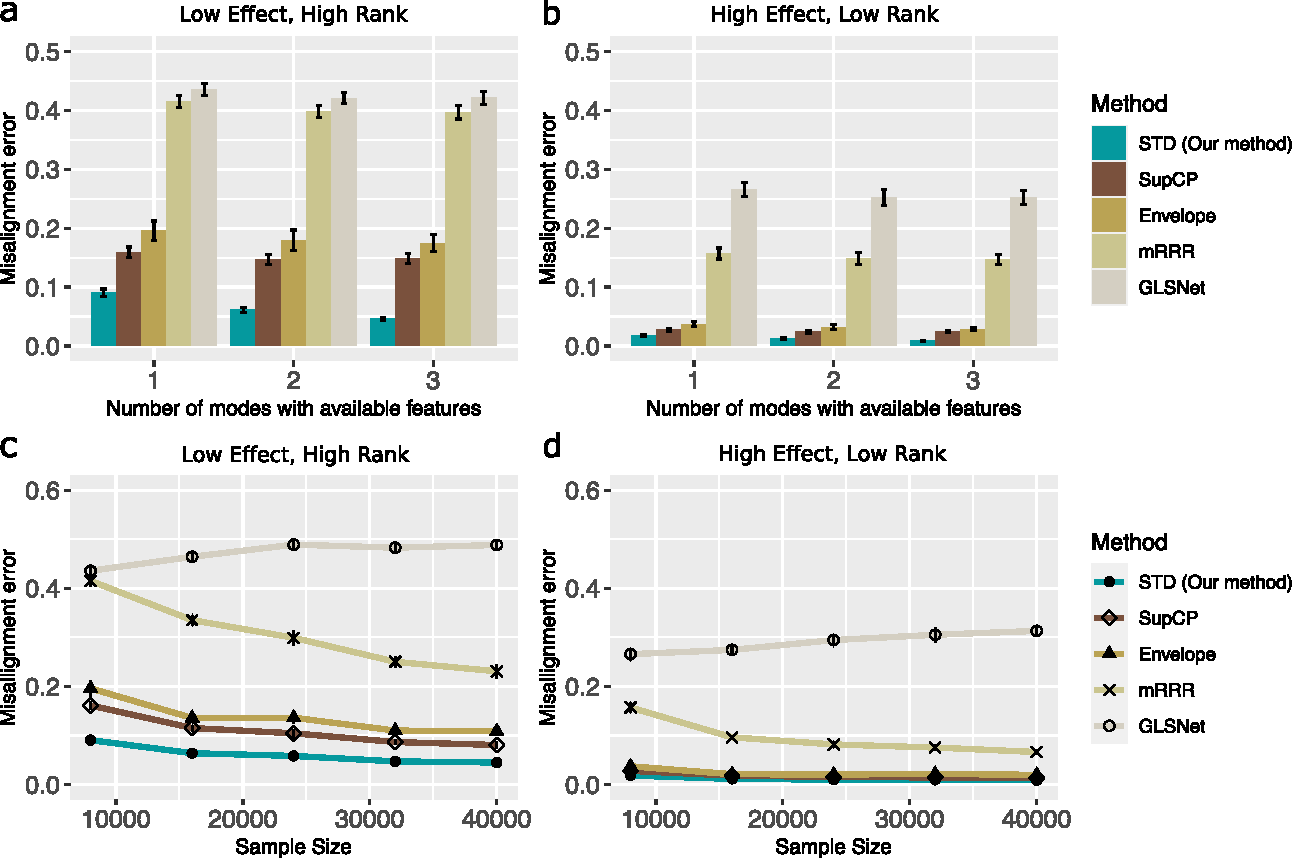
\includegraphics[width=12cm]{comp_final_normal.pdf} 
\caption{Comparison between tensor methods with Gaussian data. Panels (a) and (b) plot estimation error versus the number of modes with available features. Panels (c) and (d) plot ME versus the effective sample size $d^2$.
We consider rank $\mr=(3,3,3)$ (low), $\mr=(4,5,6)$ (high), and signal $\alpha =3 $ (low), $\alpha=6$ (high).}~\label{fig:comp}
\end{figure}

Figure~\ref{fig:comp}a-b shows the impact of features to estimation error. We see that our \textbf{STD} outperforms others, especially in the low-signal high-rank setting. As the number of informative modes increases, the \textbf{STD} exhibits a reduction in error whereas others remain unchanged. The accuracy gain in Figure~\ref{fig:comp} demonstrates the benefit of incorporating informative features from multiple modes. In addition, we find that the relative performance among the competing methods reveals the benefits of low-rankness. 
The second best method is \textbf{SupCP} which imposes low-rankness on three modes; the next one is \textbf{Envelope} which imposes low-rankness on two modes; the less favorable one is \textbf{mRRR} which imposes low-rank structure on one mode only; the worst one is \textbf{GLSNet} which imposes sparsity but no low-rankness on the feature effects. 

Figure~\ref{fig:comp}c-d compares the prediction error with respect to effective sample size $d^2$. For fair comparison, we consider the setting with feature matrix on one mode only. We find that our \textbf{STD} method has similar performance as \textbf{Envelope} and \textbf{SupCP} in the high-signal low-rank regime, whereas the improvement becomes more pronounced in the low-signal high-rank regime. The latter setting is notably harder, and our \textbf{STD} method shows advantage in addressing this challenge. Among other methods, \textbf{Envelope}, \textbf{SupCP}, and \textbf{mRRR} show decreasing errors as $d$ increases, implying the benefits of low-rankness methods. In contrast, \textbf{GLSNet} suffers from non-decreasing error and indicates the poor fit of sparsity methods in addressing low-rank data. 

\begin{figure}[htb]
\centering
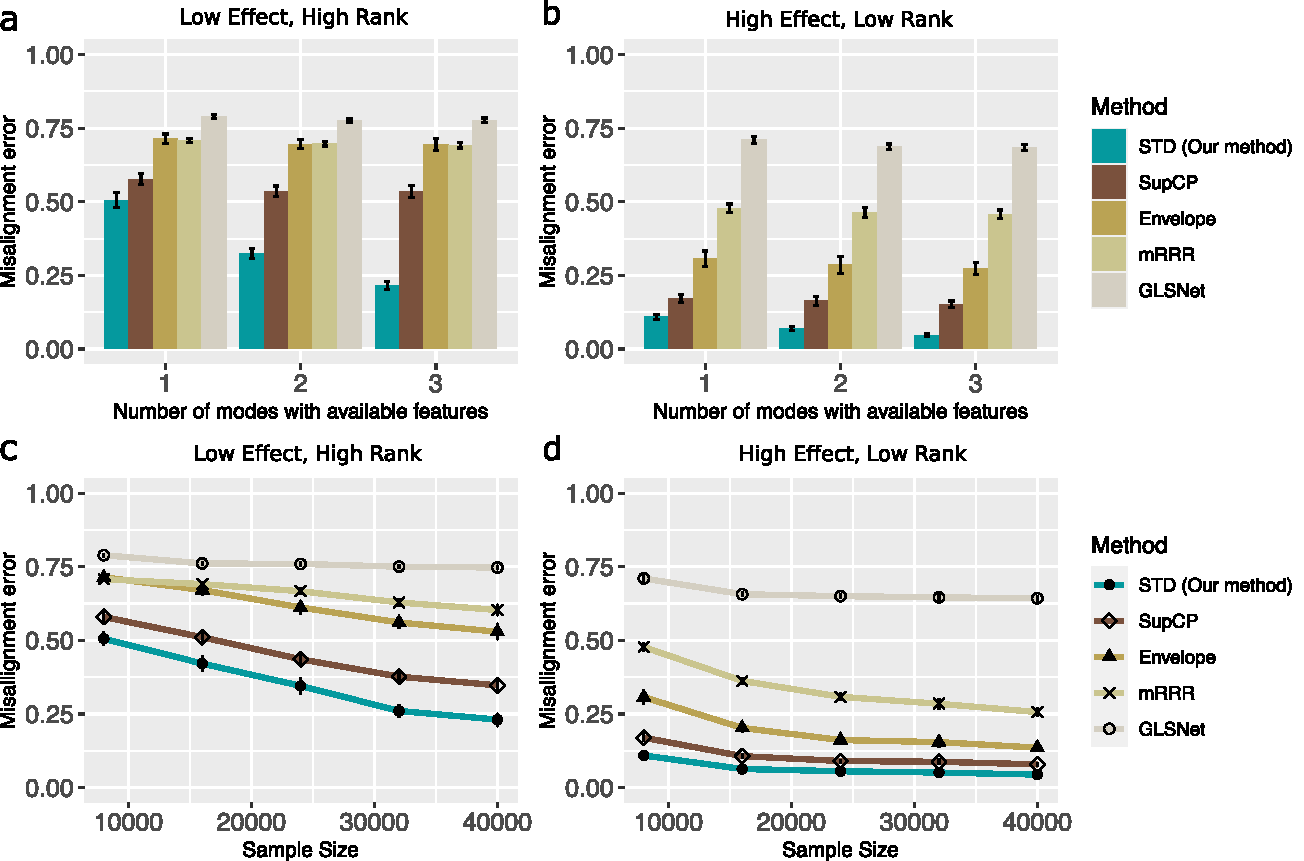
\includegraphics[width=12cm]{comp_final_binary.pdf} 
\caption{Comparison between tensor methods with Binary data. The panel legends are the same as in Figure~\ref{fig:comp}.}~\label{fig:comp_b}
\end{figure}

We also evaluate the performance comparison with Bernoulli tensors. Figure~\ref{fig:comp_b} indicates the necessarity of generalized model in addressing non-Gaussian data. Indeed, methods that assume Gaussiannity (\textbf{Envelope} and \textbf{SucCP}) perform less favorably in Bernoulli setting (Figure~\ref{fig:comp_b}c) compared to Gaussian setting (Figure~\ref{fig:comp}c). Our method shows improved accuracy as the number of informative features increases (Figure~\ref{fig:comp_b}a-b). In the absence of multiple features, our method still performs favorably compared to others (Figure~\ref{fig:comp_b}c-d), for the same reasons we have argued in Gaussian data. ''
  \end{quote}
        
        \item we have added a new experiment in Section~\ref{sec:simulation} to evaluate the robustness of our method with model misspecification:
        \begin{quote}
            ``Lastly, we assess the performance of our method {\bf STD} under model misspecification. We consider two aspects: (i) non-independent noise, and (ii) sparse feature effects. Note that our method {\bf STD} imposes neither of these two assumptions, so the experiment allows us to assess the robustness. We select competing methods from Table~\ref{table:comp_table} that specifically addresses these two aspects. We use {\bf Envelope} and {\bf SupCP} as benchmark for noise correlation experiment, and {\bf GLSNet} for sparsity experiment.

Figure~\ref{fig:noniid}a-b assesses the impact of noise correlation to the estimation accuracy. The data is simulated from {\bf Envelope} model with envelope dimensions $r=(3,3)$ (low) and $(4,5)$ (high). The noise is generated from a zero-mean Gaussian tensor with Kronecker structured covariance; see Supplementary Notes for details. As expected, {\bf Envelope} shows the best performance in the high correlation setting. Remarkably, we find that our method {\bf STD} has comparable and sometimes better performance when noise correlation is moderate-to-low. In contrast, {\bf SupCP} appears less suitable in this setting. Although {\bf SupCP} allows noise correlation implicitly through latent random factors, the induced correlation may not belong to the Kronecker covariance structure in the simulation. 



Figure~\ref{fig:noniid}c-d assesses the impact of sparsity to estimation performance. We generate data from {\bf GLSNet} model, except that we modify the coefficient tensor to be joint sparse and low-rank (the original {\bf GLSNet} model assumes full-rankness on the coefficient tensor). 
The sparsity level ($x$-axis in Figure~\ref{fig:noniid}c-d) quantifies the proportion of zero entries in the coefficient tensor. Since neither our method {\bf STD} nor {\bf GLSNet} follow the simulated model, this setting allows a fair comparison. We find that our method outperforms {\bf GLSNet} in the low-rank setting, whereas {\bf GLSNet} shows a better performance in the high-rank setting. This observation suggests the robustness of our method to sparsity when the tensor of interest is simultaneously low-rank and sparse. When sparsity is the only salient structure, then methods specifically addressing sparsity would provide a better fit.''


\begin{figure}[htb]
\centering
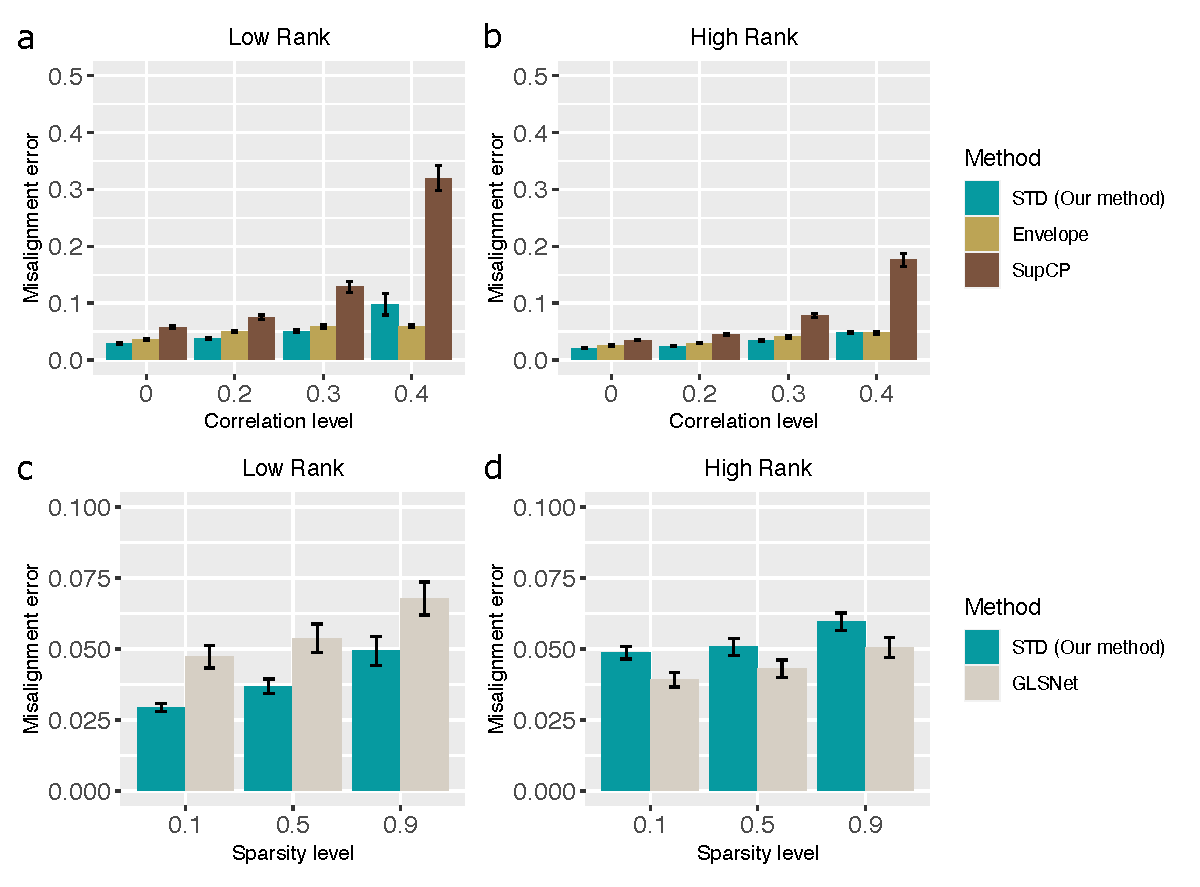
\includegraphics[width=12cm]{noniid_final.pdf} 
\caption{Comparison between tensor methods under model misspecification. Panels (a)-(b) assess the error correlation, and panels (c)-(d) assess the sparsity. }~\label{fig:noniid}
 \end{figure}
 
 \end{quote}
 
 For self-consistency, we quote the detailed simulation setups for the Figure~\ref{fig:noniid} in the Supplementary Notes, Section \ref{sec:asimulation}:
\begin{quote}
    ``
    \textbf{B.1 Detailed simulation setup for Figure~\ref{fig:noniid}a-b}
    
    \vspace{0.2cm}
    
    We generate data from \textbf{Envelope} model \citep{li2017parsimonious} with slight modification. We simulate response tensor $\tY\in\mathbb{R}^{d\times d\times d}$ from the following model with envelope dimension $(u_1, u_2)$,
\begin{align}\label{eq:e}
    \tY|\mX &= \tB \times_3 \mX + \tE = \tC \times \{\mGamma_1, \mGamma_2,\mX\}+ \tE, \notag \\
    \text{with} \quad \tE &\sim \mathcal{TN}(\mSigma_1, \mSigma_2, \mI), \quad \mSigma_k = \mGamma_k \mOmega_k \mGamma_k^T + \mGamma_{0k} \mOmega_{0k} \mGamma_{0k}^T+\mI, \quad k = 1,2,
\end{align}
 where $\mX\in\mathbb{R}^{d\times p}$ is the feature matrix, $\tB=\tC\times\{\mGamma_1,\mGamma_2, \mI\}\in \mathbb{R}^{d\times d\times p}$ is the coefficient tensor, $\tC\in\mathbb{R}^{\mu_1\times \mu_2\times p}$ is a full-rank core tensor, $\mathcal{TN}(\cdot,\ \cdot,\ \cdot)$ represents zero-mean tensor normal distribution with Kronecker structured covariance, 
 $\mGamma_{k} \in \mathbb{O}(d,u_k)$ 
 consists of orthogonal columns, $\mGamma_{0k} \in \mathbb{O}(d,d-u_k)$ is the orthogonal complement of $\mGamma_k$, and  $\mOmega_k = \mA_k\mA_k^T$, $\mOmega_{0k} = \mA_{k0}\mA_{k0}^T$ with $\mA_k \in \bbR^{u_k \times u_k}$,  $\mA_{k0} \in \bbR^{(d - u_k) \times (d - u_k)}$. 
 
 The entries of $\mX$ are i.i.d.\ drawn from $\tN(0,1)$, the entries of $\mA_k$, $\mA_{k0}$ are i.i.d.\ drawn from $\textup{Uniform}[-\gamma, \gamma]$, and the entries of core tensor $\tC$ are i.i.d.\ drawn from $\textup{Uniform}[-3,  3]$. We call $\gamma$ the \textit{correlation level}. Note that the only distinction between model~\eqref{eq:e} and standard {\bf Envelope} model is the additional identity matrix $\mI$ in the expression of $\mSigma_k$. When $\gamma = 0$, the model~\eqref{eq:e} reduces to our \textbf{STD} model with rank $\mr = (u_1,u_2,p)$. We set $d=20, p=5$ in our simulation.  
 
 \vspace{0.2cm}
 \textbf{B.2 Detailed simulation setup for Figure~\ref{fig:noniid}c-d}
 
 \vspace{0.2cm}
 
We generate the data from  \textbf{GLSNet} model \citep{zhang2018network} with slight modification. We simulate the binary response tensor $\tY \in \{0,1\}^{d \times d \times d}$ from the following model
\begin{align}
    \mathbb{E}[\tY|\mX] = f({\bf 1} \otimes {\bf \Theta} + \tB \times_3 \mX),
\end{align}
where $f(\cdot)$ is the logistic link, $\mX \in \mathbb{O}(d,p)$ is the feature matrix with orthonormal columns, ${\bf \Theta}=\mA \mA^T \in \bbR^{ d \times d }$ is a rank-$R$  intercept matrix, where the entries of $\mA \in \bbR^{d \times R}$ are simulated from i.i.d.\ standard normal. 
Unlike original \textbf{GLSNet} model, we generate joint sparse and low-rank structure to the coefficient tensor $\tB$ as follows. 

To generate $\tB$, we firstly generate a low-rank tensor $\tB_0$ as 
\begin{align}
    \tB_0 = \tC \times \mM_1 \times \mM_2 \times \mM_3,
\end{align}
where $\tC \in \bbR^{R \times R \times R}$ is a full-rank core tensor, $\mM_1, \mM_2 \in \bbR^{d \times R}$ and $\mM_3 \in \bbR^{p \times R}$ are the factor matrices with orthonormal columns. We simulate i.i.d.\ uniform entries in $\tC$ and rescale the tensor $\tB_0$ such that $\onorm{\tB_0}_{\max} = 2$. Last, we obtain a sparse $\tB$ by randomly setting $sd^2p$ entries in $\tB_0$ to zero. We call $s$ the \textit{sparsity level} which quantifies the proportion of zero's in $\tB$. Hence, the generated tensor $\tB$ is of sparsity level $s$ and of low-rank $(R,R,R)$. We set $d = 20$, $p = 5$ and consider the combination of rank $R = 2$ (low), $4$ (high) and sparsity level $s = \{0, 0.3,0.5\}$ in the simulation. "

\end{quote}
 
 
\end{enumerate}

    \item \textit{Additional discussion on side information should be included that involves i) how do we know in practice if side information is appropriate; ii) dimensionality of the side information.}
    
    \vspace{0.2cm}
    \textbf{Response:} See our response to \textbf{\# 5, Reviewer 2}.
    
    \item \textit{The authors should discuss initialization and how to obtain the initial error condition. Can something be said about the proposed random initialization in Algorithm 1?} 
    
         \textbf{Response:} We have added theoretical justifications to two initializations. See our response {\bf \# Initialization, Reviewer 1.} 
         
    \item \textit{There is a disconnect between the proposed algorithm and established theory. Can the authors establish statistical properties for the iterative algorithm? If not, what are the technical challenges that are not present in the related literature?}
    
     \textbf{Response:} We have added new theory to establish the accuracy for both (i) global MLE and (ii) local optimizer. See our response to {\bf \# Theoretical Studies, Reviewer 1.}
    
    \item \textit{Some discussion on the computationally tractable selection of ranks should be included. See comment from Reviewer 2.}
    
    \textbf{Response:} We have added more detailed discussions and reported the running time for rank selection. See our response to \textbf{\# 8, Reviewer 2}.
\end{enumerate}

\newpage

\begin{center}
    \textbf{Point-by-point Response to Reviewer 1}
\end{center}

We greatly appreciate your valuable comments and suggestions. We have carefully addressed all the questions. Note that general comments raised by both reviewers were addressed upfront in {\bf pages 1-7 of this response letter, Response to Major Comments Summarized by Editor}. We will make explicit reference to earlier section when needed. 

\vspace{0.2cm}

\textit{This paper introduces a novel supervised tensor decomposition model when there are side information on multiple modes. This model can be viewed as an extension to tensor response regression. As compared to existing tensor response regression models \citep{rabusseau2016low,li2017parsimonious,sun2017store}, the proposed method has three advantages. First, it allows covariate information on multiple modes instead of one mode. Second, it allows high-dimensionality on both the tensor size $d_k$ and covariate size $p_k$. Third, it allows a flexible data type of the tensor, including continuous, count, and binary observations. Data satisfying these properties are not rare, and the paper has provided three data examples. Therefore, I believe this is a useful and well-motivated work. The construction of the estimator leads to a non-convex optimization. Both algorithm and theoretical study are constructed. This work can be regarded as a non-trivial extension of these tensor response regression models as well as \cite{wang2020learning} on probabilistic tensor decomposition which decomposes a tensor with continuous, count, or binary observations. Overall, I think this is an interesting work that has potential usefulness and will contribute to the literature of tensor regression. I enjoy reading the paper and feel it would be suitable for JCGS if the following comments are addressed. I recommend a major revision.}

\vspace{0.2cm}
\textit{\textbf{Initialization:}}
\begin{enumerate}[wide, labelwidth=!, labelindent=0pt]
    \item \textit{How to initialize to achieve the initial error condition, as stated in Proposition 4.1 (Global convergence)?}
    
    {\bf Response:} We recommend two schemes for initialization: random initialization (cold start) and spectral initialization (warm start). In the high signal-to-noise regime, we have added theoretical guarantees for the statistical accuracy of warm start within polynomial running time. In the low signal-to-noise regime, the statistical-computational gap arises in which case random initialization often provides better empirical results. {\bf We have added a new section for provable initialization and its implementation.} See our detailed response to  {\bf\# Theoretical Studies}.    
    
    We have added the following paragraph in Section~\ref{sec:rankM}:
    \begin{quote}
    ``...We provide two initialization schemes, one with QR-adjusted spectral initialization (warm initialization), and the other with random initialization (cold initialization). The warm initialization is an extension of unsupervised spectral initialization~\citep{zhang2018tensor} to supervised setting with multiple feature matrices. ... The initialization scheme is described in Algorithm~\ref{alg:A}. 

The warm initialization enjoys provable accuracy guarantees at a cost of extra technical assumptions (see Section~\ref{subsec:statprob}). The cold initialization, on the other hand, shows robust in practice but its theoretical guarantee remains an open challenge~\citep{luo2021low}. We incorporate both options in our software package to provide flexibility to practitioners...''
\end{quote}

\begin{algorithm}[!h]
\caption{QR-adjusted spectral initialization}\label{alg:A}
\begin{algorithmic}[1]
\INPUT Response tensor $\tY\in \mathbb{R}^{d_1\times \cdots \times d_K}$, feature matrices $\mX_k\in\mathbb{R}^{d_k\times p_k}$, Tucker rank $\mr$. 
\State Normalize date tensor $\bar \tY\leftarrow \tY$ for Gaussian model, $\bar \tY\leftarrow 2\tY-1$ for Bernoulli model, and $\bar \tY\leftarrow \log(\tY+0.5)$ for Poisson model. 
\State Normalize feature matrices via QR factorization $\mX_k=\mQ_k\mR_k$ for all $k\in[K]$.
\State Obtain $\bar \tB \leftarrow \bar \tY\times\{\mQ^T_1,\ldots,\mQ^T_K\}$ by projecting $\bar \tY$ to the multilinear feature space. 
\State Obtain $\hat\tB^{(0)}\leftarrow \textup{HOSVD}(\bar \tB,\mr)$.
\State Normalize representation $\{\hat\tC^{(0)}, \hat\mM^{(0)}_1,\ldots,\hat\mM^{(0)}_K\}$ such that $\hat\tC^{(0)}\times\{ \hat\mM^{(0)}_1,\ldots,\hat\mM^{(1)}_K\} = \hat\tB^{(0)}\times\{ \mR^{-1}_1,\ldots,\mR^{-1}_K\}$ and $\hat\mM^{(0)}_k\in\mathbb{O}(p,r)$ for all $k\in[K]$.
\OUTPUT Core tensor $\hat\tC^{(0)}$ and factors $\hat\mM^{(0)}_k$ for all $k\in[K]$.
\end{algorithmic}
\end{algorithm}
    
    \item  \textit{As the proposed estimator is obtained from a nonconvex optimization, the possibility of having multiple local optimizers is a problem. In Algorithm 1, a random initialization is used. Can the authors construct an empirical study of how serious the local optimal affects the statistical performance of the randomly initialized estimator? Does the random initialization always lead to the global optimum?}
    
     \textbf{Response:} The empirical performance of random initialization was investigated in Figure~\ref{fig:loglike} in the original paper and the remarks thereof. We have shown in Theorem~\ref{thm:MLE} that the same statistical rate holds, not only for the {\it global optimizer}, but also for every {\it local optimizer} with sufficiently large objective values. In this sense, local optimality is not necessarily a severe concern in our context. We have added the following sentences for clarification in Sections~\ref{sec:global} and Section~\ref{sec:local}: 
     
     \begin{quote}
         ``...Inspection of our proof (Supplementary Notes) shows that the desired convergence rate holds not only for the MLE, but also for all local optimizers in the set $\tL_{\tY}(\tC, \mM_1,\ldots,\mM_K)\geq \tL_{\tY} (\tC_{\textup{true}},\mM_{1,\textup{true}},\ldots,\mM_{K,\textup{true}})$. The observation indicates the global optimality is not necessarily a serious concern in our context, as long as the convergent objective is large enough. In next section, we will provide the statistical accuracy for \emph{local} optimizer with provable convergence guarantee, at a cost of extra signal requirement...''
     \end{quote}
     
     \begin{quote}
     ``...We supply the theory by providing an alternative scheme -- random initialization -- and investigate its empirical performance. Figure~\ref{fig:loglike} shows the trajectories of objective function ... In the experiment we conduct, we find random initialization appears good enough for Algorithm~\ref{alg:B} to find a convergent point with desired statistical guarantees. In practice, we recommend to run both warm and cold initializations, and choose the one with better convergent objective values...''
     \end{quote}
     
     
     On a related note, characterizing the optimization landscape and impact of initialization are problems of interest. Inspired by the reviewer's comment, {\bf we have added new theory for provable initialization and per-iteration accuracy.} See our response to {\bf\# Theoretical Studies}. 
    
     
     \begin{quote}


\end{quote}
     
\end{enumerate}

\vspace{0.2cm}
\textit{\textbf{Theoretical Studies:}}

\begin{enumerate}[wide, labelwidth=!, labelindent=0pt]
    \item \textit{The statistical properties established in Theorem 4.1 is for the M-estimator in (8). However, due to non-convexity of this optimization, the maximizer of (8) may not be achievable by practical algorithms. Therefore, it would be more convincing to prove statistical properties for the iterative estimator from the alternating optimization in Algorithm 1. Such theorem is pretty standard in recent tensor regression models with low-rank structure \citep{sun2017store, raskutti2019convex,hao2019sparse,han2020optimal}. If this proof is not possible, it would be helpful if the authors could discuss the technical challenges.}
  
    
    {\bf Response: }Thank you for the suggestion. Inspired by your comments, we have now proved the statistical properties for the iterative estimator from the alternating optimization in Algorithm 1. We summarize the new results below; the detailed revisions are in Section~\ref{subsec:statprob}. 
    
     \begin{quote}
    ``...This section presents the accuracy guarantees for both global and local optimizers of~\eqref{eq:MLE}. We first provide the statistical accuracy for the global MLE~\eqref{eq:MLE}. Then, we provide the convergence rate for the local optimizer from Algorithm~\ref{alg:B} with warm initialization. The rate reveals an interesting interplay between statistical and computational efficiency. We show that a polynomial number of iterations suffices to reach the desired accuracy under certain assumptions...'' 
    \end{quote}
    
     \begin{quote}
``...Under mild conditions, our warm initialization enjoys stable performance, and the subsequent iterations further improve the accuracy via linear convergence; i.e.\ sequence of iterates generated by Algorithm~\ref{alg:B} converges to optimal solutions at a linear rate. 

\begin{prop}[Polynomial-time angle estimation]\label{lem:ini} Consider Gaussian tensor models with $b(\theta)=\theta^2/2$ in the objective function~\eqref{eq:loglikelihood}. Suppose the signal-to-noise ratio $\lambda^2/\phi \geq C p^{K/2}d^{-K}$ for some sufficiently large universal constant $C>0$. 
Under Assumption A1 with scaled feature matrices $\bar \mX_k=\sqrt{d}\mX_k$, or Assumption A1' with original feature matrices, the outputs from initialization Algorithm~\ref{alg:A} and iteration Algorithm~\ref{alg:B} satisfy the following two properties.
\begin{enumerate}[label=(\alph*)]
\item With probability at least $1-\exp(-p)$. 
\begin{equation}\label{eq:warm}
\max_{k\in[K]}\sin^2\Theta(\trueM,\hat \mM_k^{(0)})\leq {1\over 4}. 
\end{equation}
\item Let $t=1,2,3,\ldots,$ denote the iteration. There exists a contraction parameter $\rho\in(0,1)$, such that, with probability at least $1-\exp(-p)$, 
\begin{equation}\label{eq:local}
\max_{k\in[K]}\textup{sin}^2 \Theta(\trueM, \hat \mM^{(t)}_k) \lesssim \KeepStyleUnderBrace{{\phi p \over \lambda^2 d^K}}_{\text{statistical error}}+\KeepStyleUnderBrace{\rho^{t}\max_{k\in[K]}\textup{sin} \Theta^2(\trueM, \hat \mM_k^{(0)})}_{\text{algorithmic error}}.
\end{equation}
\end{enumerate}
\end{prop}

Proposition~\ref{lem:ini} provides the estimation errors for algorithm outputs at initialization and at each of the subsequent iterations. The initialization bound~\eqref{eq:warm} demonstrates the stability of QR-adjusted spectral initialization under a mild SNR requirement $\lambda^2/\phi \gtrsim p^{K/2}d^{-K}$. We can think of $d$ as the sample size while $p$ the number of parameters at mode $K$. The condition confirms that a higher sample size mitigates the required signal level. The iteration bound~\eqref{eq:local} consists of two terms: the first term is the statistical error, and the second is the algorithmic error. The algorithmic error decays exponentially with the number of iterations, whereas the statistical error remains the same as $t$ grows. The statistical error is unavoidable and also appears in the global MLE; see Theorem~\ref{thm:MLE}.

As a direct consequence, we find the optimal iteration $t$ after which the algorithmic error is negligible compared to statistical error. 
\begin{thm}[Statistical rate for local optimizers]\label{thm:local}Consider the same condition as in Proposition~\ref{lem:ini} and the outputs by combining algorithms 1 and 2. There exists a constant $C>0$, such that, after $t\gtrsim K\log_{1/\rho}p$ iterations, our algorithm outputs satisfies
\[
\max_{k\in[K]}\textup{sin}^2 \Theta(\trueM, \hat \mM^{(t)}_k) \lesssim {\phi p\over \lambda^2d^K}, \quad \FnormSize{}{\trueB- \hat \tB^{(t)}}^2 \lesssim {\phi(r^K+Kpr)\over d^K}.
\]
\end{thm}


In practice, the signal level $\lambda$ is unknown, so the assumption in Theorem~\ref{thm:local} is challenging to verify in practice. We supply the theory by providing an alternative scheme -- random initialization -- and investigate its empirical performance...''
    
    \end{quote}
    
    \item \textit{As shown in Theorem 4.1, the rate of convergence is in the order $\sum_k p_k/ \prod_k d_k$ when other terms fixed. Here $p_k$ is the covariate size along $k$-th mode. I am curious if there is any insight on the optimality of this scaling. Since handling multiple covariates is one of the key contributions of this work, I think more discussion of the order of $p_k$ would be useful. For instance, it would be helpful to compare this rate with the optimal rate established in tensor regression \citep{han2020optimal} and probabilistic tensor decomposition \citep{wang2020learning}. }
    
    {\bf Response:} We have explained the intuition about our optimality and the benefit of incorporating multiple feature matrices. We added discussions to the scaling factors in Section~\ref{subsec:statprob}:
    

\begin{quote}
``...The result in~\eqref{eq:bound} implies that the estimation has a convergence rate $\tO(Kp/d^{K})$...This rate agrees with intuition, since in our setting, the number of parameters with $K$ feature matrices is of order $\tO(Kp)$, whereas the number of tensor entries $\tO(d^K)$ corresponds to the total sample size. Because $p\leq d$, our rate is faster than $\tO(d^{-(K-1)})$ obtained by tensor decomposition without features~\citep{wang2020learning}..''

``...The initialization bound~\eqref{eq:warm} demonstrates the stability of warm initialization under a mild SNR requirement $\lambda^2/\phi \gtrsim p^{K/2}d^{-K}$. We can think of $d$ as the sample size while $p$ the number of parameters at mode $K$. This threshold is less stringent than $d^{K/2}$ required for tensor decomposition without multiple features~\citep{han2020optimal,zhang2018tensor}...''
\end{quote}
\end{enumerate}

\vspace{0.2cm}
\textit{\textbf{Numerical comparison:}}
\begin{enumerate}
    \item \textit{In Section 5.2 (simulation) and Section 6.1 (HCP data), only the multiple-response GLM method is compared. This setting seems to be a special case of the network response regression \citep{zhang2018network}, therefore it would be interesting to add it in the comparison. If they are not directly comparable, it would be helpful to discuss it.}
    
    \textbf{Response:} We have added comparison with 12 methods, including GLSNet~\citep{zhang2018network}, in the new Section~\ref{sec:connection}. For alternative methods in numerical analysis, we have also replaced the earlier old methods by more recent methods, including~\cite{zhang2018network}, in Section~\ref{sec:simulation}. See our response to \textbf{\# 1, Major Comments Summarized by Editor} for full details. 
    

    \item \textit{There are other recent tensor response regression models \citep{li2017parsimonious,sun2017store,raskutti2019convex}. Some of them are missing in the paper. It would be interesting to see the comparison with more recent tensor response regression models in Section 5.3. If they are not directly comparable, it would be helpful to discuss it.}
    
    \textbf{Response:} We have made changes as suggested. Comparisons are summarized in our response to \textbf{\# 1, Major Comments Summarized by Editor}. 
\end{enumerate}

\vspace{0.2cm}
\textit{\textbf{Minor issues and typos:}}

\begin{enumerate}
     \item \textit{The notation $\alpha$ is used for both the maximum norm constraint on page 13, and the signal level on page 19. Are they same? If not, it would be helpful to use different notations.}
        
         \textbf{Response:} 
        They are the same. The sentence now reads:
         \begin{quote}
             ``... Here $\alpha>0$ controls the magnitude of the effect size, which is also the maximum norm of coefficient tensor as in~\eqref{eq:p}...."
         \end{quote}
         
    \item \textit{In the optimization (8), the authors add a maximum norm constraint on the linear predictor to avoid the divergence in the non-Gaussian variance. Can authors provide more explanations on this constraint? } 
    
    \textbf{Response:} We have added the following explanation in Section~\ref{sec:rankM}:
    \begin{quote}
       ``...The maximum norm constraint on the linear predictor $\Theta$ is a technical condition to ensures the existence (boundedness) of MLE. 
The condition precludes the ill-defined MLE when the optimizer of~\eqref{eq:MLE} diverges to $\pm \infty$; this phenomenon may happen in logistic regression when the Bernoulli responses $\{0,1\}$ are perfectly separable by covariates~\citep{wang2020learning}. For Gaussian models, no maximum norm constraint is needed. In Section~\ref{subsec:statprob}, we show that setting $\alpha$ to an extremely large constant does not compromise the statistical rate in quantities of interest. In practice, the unbounded search is often indistinguishable from the bounded search, since the boundary constraint $\onorm{\Theta}_{\infty} \leq \alpha$ would likely never be active. Similar techniques are commonly used in high-dimensional non-Gaussian problems~\citep{wang2020learning,han2020optimal}...''
    \end{quote}
    
     \item \textit{What’s the tuning range for the ranks $r_1,...,r_K$ in the experiments?}
     
     \textbf{Response:} 
     For simulation, we have added the following details in Section~\ref{sec:simulation}:
     \begin{quote}
         ``...For each combination, we minimize BIC using a grid search from $(r_1-3, r_2-3, r_3-3)$ to $(r_1+3, r_2+3, r_3+3)$. We remove invalid rank combinations such as $r^2_{\max} \geq \prod_{k=1}^3 r_k$ and use parallel search to reduce the computational cost....'' 
     \end{quote}
         
 For data application, we have added the following clarification in Section~\ref{sec:data}. Detailed rank selection is provided in a new section {\bf Rank selection for Nations data, Supplementary Notes}. 
   \begin{quote}
   ``... We use BIC as guidance to select the rank of coefficient tensor $\tB$. Since several rank configurations give similar BIC values, we present here the most interpretable results with $\mr=(4,4,4)$. Detailed rank selection procedure is in Supplementary Notes...''
\end{quote}

\item \textit{Typos: 1) line -3 on page 18, $\mM_2 \mX_3$ should be $\mM_2\mX_2$; 2) Table 2, the column names $d = 20$ and $d = 40$ are missing.} 

\textbf{Response:} We have made the correction as suggested.

 
\end{enumerate}

\clearpage
\newpage

\begin{center}
    \textbf{Point-by-point Response to Reviewer 2}
\end{center}

We greatly appreciate your valuable comments and suggestions. We have carefully addressed all the questions. Note that general comments raised by both reviewers were addressed upfront in {\bf pages 1-7 of this response letter, Response to Major Comments Summarized by Editor}. We will make explicit reference to earlier section when needed. 

{\it The paper develops a Tucker decomposition technique for tensor data, which can consider side information in each mode. In particular, the model is built upon the exponential family to handle non-Gaussian data, and the method is formulated as a generalized tensor regression problem. An alternating algorithm is proposed to estimate the model parameters. The statistical convergence is derived for the proposed method. The applications to a brain imaging example and an international relation example reveal some interesting structures in data. Overall, the paper is well written and easy to read. The numerical results demonstrate the potential utilities of the proposed method. There are a few places where the paper can be further improved. }


\begin{enumerate}[wide, labelwidth=!, labelindent=0pt]
    \item \textit{The term “interactive” is used in the title and throughout the paper. However, it is not very clear from the paper what it means to be interactive. It seems the side information is always assumed given and static. In that case, I would recommend removing the term. }
    
    \textbf{Response:} We have removed the term as suggested. 
    
    \item \textit{There are quite a few non-Gaussian tensor models for various analyses in the literature \citep{tarzanagh2019regularized, li2020generalized, chi2012tensors, hong2020generalized}. A more thorough literature review is warranted. }
    
    \textbf{Response:} Thank you for pointing out the related literature. The methods \citep{chi2012tensors, hong2020generalized} were reviewed and compared in the first version. We have added detailed literature discussions with 12 more methods and the numerical comparisons. See our response to \textbf{\# 1, Major Comments Summarized by Editor} for the full comparison.     
        
    \item \textit{The proposed method is closely related to the envelope model (especially for Gaussian data)\citep{li2017parsimonious}. It would be of interest to discuss the similarity and difference between the two.}
    
    \textbf{Response:} Per reviewer's suggestion, we have added more literature reviews and updated the numerical comparisons. See our response to, \textbf{\# 1, Major Comments Summarized by Editor}. 
    
    
    
    \item \textit{The dimension requirements seem unnecessarily strong. In particular, the number of features in the side information ($p_k$) is required to be smaller than the dimension of the corresponding mode of the tensor data ($d_k$); the rank of the core tensor ($r_k$) needs to be smaller than $p_k$. In practice, how to handle a large number of features (i.e., $p > d$)? If the number of features is small (e.g., in the HCP example, there are only 2 individual features where age is further discretized as dummy variables), can the rank of the core tensor exceed the feature dimension? More discussions are needed.}
    
    \textbf{Response:} There are two questions here, one on $r\leq p$, and the other on $p\leq d$. We discuss them separately. 
    
  {\bf Regarding the condition $r\leq p$.} This is not a requirement but rather a natural fact based on definition of tensor rank.  Notice that $p$ is the dimension of parameter tensor of interest, and $r$ is the rank of the parameter tensor. Numerically, one must have $r\leq p$; i.e, the rank of core tensor cannot exceed the feature dimension. 
  
 From the modeling perspective, the fact $r\leq p$ comes from the goal of the problem: we aim to identify tensor factors that are most attributable to features. In the HCP example, our goal is to find the relationship between data tensor  $\tY\in\{0,1\}^{68\times 68\times 136}$ and the feature $\mX\in\mathbb{R}^{4\times 136}$. The fullest linear model has coefficient $\tB\in\mathbb{R}^{68\times 68\times 4}$, with rank upper bounded by 4 on the last mode. 

  
{\bf Regarding the condition $p\leq d$.} This condition requires the feature to have full column rank. We view it as a mild condition, because same condition is also imposed in classical linear regression. In the presence of rank deficiency, we recommend to remove redundant features before applying our method. 

We have added more discussions in Sections~\ref{sec:model} and~\ref{subsec:statprob}. 
\begin{quote}
        ``..the identifiability of $\tB$ requires the feature matrices $\mX_k$ are of full column rank with $p_k\leq d_k$. We impose this rank non-deficiency assumption to $\mX_k$; this is a mild condition common in literature~\citep{lock2018supervised, li2017parsimonious, li2020generalized}. In the presence of rank deficiency, we recommend to remove redundant features from $\mX_k$ before applying our method. ..."
\end{quote}
  \begin{quote}
  ``...the requirement $p\leq d$ is necessary to ensure rank non-deficiency of  feature matrices $\mX_k$..''
  \end{quote}
    
\item \textit{A related question to the above comment: if the side information is little (small $p_k$) or irrelevant to the underlying structure of the tensor data, would the proposed model structure (3) be overly restrictive rather than helpful? In other words, the “supervised tensor factor” $\mX_k\mM_k$ must reside in the column space of the features $\mX_k$. If $\mX_k$ is not well selected, would that lead to a biased decomposition of the original data? In practice, how do we know if a set of features are appropriate to use? The envelope model \citep{li2017parsimonious,lock2018supervised} may offer an alternative perspective by separating the data variation into a material part (related to $\mX_k$) and an immaterial part (irrelevant to $\mX_k$). It’s not clear whether the idea directly applies to the proposed method in this paper since the low-rank model is on the deterministic mean tensor. Some discussions would be helpful.}
    
    \textbf{Response:} We agree with the basic premise of the reviewer that the our method relies on the choice of feature matrices. In fact, this does not undermine our method's utility. A major point we want to make in response is that the goal of our problem is to estimate the {\it conditional pattern} of $\tY|\mX$, not the {\it overall pattern} of $\tY$. This motivation has guaranteed the validness (unbiasedness) of our factors, even when the $\mX$ is poorly related to $\tY$. The tensor factors we learned are not intended to explain the most variation in the $\tY$; instead, they are intended to capture the variation that is most attributable to features. 
    
    There are methods that jointly impose data variation in conditional component $\tY|\mX$ and residual component $\tY-\tY|\mX$. These methods have the benefits of joint learning the conditional variation of $\mathbb{E}(\tY|\mX)$ and the variation of residuals. The referred methods, Envelope~\citep{li2017parsimonious} and SupCP~\citep{lock2018supervised}, fall into this category. We have added connection and comparison with these two methods in  Section~\ref{sec:connection} and in Section~\ref{sec:simulation}. See our response to {\bf \# 1, Major Comments Summarized by Editor}. 

For reviewer's interest, we discuss the practical guidance about ``which method should we use.'' 
\begin{enumerate}
    \item In general, the answer depends on the goal and problem at hand. If the goal is to identify the relationship between tensor data $\tY$ and features $\mX$, then we would recommend our method. In the three examples  illustrated in Section~\ref{sec:motivation} and two data applications in Section~\ref{sec:data}, we are interested in identifying the relationship between data tensor ( brain connectivities, social community patterns) and available features (age, gender). In these cases, direct modeling $\tY|\mX$ yields a higher accuracy, especially when variation in $\tY|\mX$ is weak compared to the overall variation in $\tY$. 
    
    \item If the goal is to identify unknown variation in the data tensor $\tY$, then we recommend Envelope~\citep{li2017parsimonious} and SupCP~\citep{lock2018supervised}. These two methods have the benefits of separating the variations of $\tY$ into explained part by $\mX$ and unexplained part due to unmeasured latent factors. 
    
    \item If the goal is to identify the relationship between $\tY$ and $\mX$ while adjusting for latent factors, then we would recommend generalized mixed-effect tensor decomposition (MSTD). The MSTD combines the advantages of our STD method and the envelope method. We have described MSTD in the original version of Discussion, and we now elaborate the discussion in light of aforementioned work. 
    
    
    \begin{quote}
    ``(our method)...can be extended by introducing a more general mixed-effect tensor model. For example, in the special case of Gaussian model, we can model the first two moments of data tensor using
\begin{align}\label{eq:extention}
\mathbb{E}(\tY|\mX_1,\ldots,\mX_K)&=\tC\times\mM_1\times \cdots \times \mM_K,\\
 \text{Var}(\tY|\mX_1,\ldots,\mX_K)&=\mPhi_1\otimes \cdots \otimes \mPhi_K,
\end{align}
where $\mPhi_k\in\mathbb{R}^{d_k\times d_k}$ is the unknown covariance matrix on the mode $k\in[K]$. For general exponential family, an additional mean-variance relationship should also be considered. The joint estimation of mean model $\Theta$ and variance model $\mPhi_k$ will lead to more efficient estimation in the presence of unmeasured confounding effects....Suitable regularization such as .... specially-structured covariance~\citep{li2017parsimonious,lock2018supervised} should be considered...''
    \end{quote}
\end{enumerate}

    
     \item \textit{Identifiability. Is the proposed model (3) identifiable? It seems not from Definition 1 (Equivalence class). If it’s not identifiable, what benefit does the orthogonality constraint on $\mM_k$ induce? How to interpret the estimated parameters? } 
     
     \textbf{Response:} Our method is to estimate the low-rank tensor $\tB$, or equivalently, the core tensor $\tC$ and factors $\mM_k$ that forms $\tB = \tC \times \{ \mM_1,...,\mM_K \}$. The tensor $\tB$ is identifiable while the factors $\{\tC, \mM_1,...,\mM_K \}$ are not. The non-unique factors incur no concern to the interpretation, because all our parameter estimation and interpretation are about $\tB$.  
     
     The orthonormality of $\mM_k$ is imposed purely for technical convenience. This normalization incurs no impacts in our statistical inference, but may help with numerical stability in empirical optimization~\citep{de2000multilinear, kolda2009tensor}.
    
    
    We have added the following discussions in Section~\ref{sec:mainmodel} and Section~\ref{sec:global}:   
     \begin{quote}
         ``...We make several remarks about model identifiability. First, the identifiability of $\tB$ requires the feature matrices $\mX_k$ are of full column rank....Second, the decomposition $\tB = \tC\times\{\mM_1,\ldots,\mM_K\}$ are non-unique, as in standard tensor decomposition~\citep{kolda2009tensor}. For any invertible matrices $\mO_k\in\mathbb{R}^{r_k\times r_k}$, $\tB=\tC\times\{\mM_1,\ldots,\mM_K\}=\tC'\times\{\mM_1\mO_1,\ldots,\mM_K\mO_K\}$ are two equivalent parameterizations with $\tC'=\tC\times\{\mO^{-1}_1,\ldots,\mO^{-1}_K\}$ . To resolve this ambiguity, we impose orthonormality to $\mM_k\in\mathbb{O}(p_k,r_k)$ and assess the estimation error of $\mM_k$ using angle distance. The angle distance is invariant to orthogonal rotations due to its geometric definition. See Section~\ref{subsec:statprob} for more details. The orthonormality of $\mM_k$ is imposed purely for technical convenience. This normalization incurs no impacts in our statistical inference, but may help with numerical stability in empirical optimization~\citep{de2000multilinear, kolda2009tensor}.''
     \end{quote}
   
   \begin{quote}
       ``...Recall that the factor matrices $\mM_k$ are identifiable only up to orthogonal rotations. Therefore, we choose to use angle distance to assess the estimation accuracy of $\mM_k$...''
   \end{quote}
    
    \item \textit{The maximum norm constraint on the linear predictor Theta is a bit ad hoc. How to choose the upper bound $\alpha$ in practice? How does the value of alpha affect the final results? }
    
    \textbf{Response:} The maximum norm constraint is a technical condition purely for theoretical analysis. In practice, no choice of $\alpha$ is needed. 
    
    
    We have added the following explanations in Section~\ref{sec:rankM}:
    \begin{quote}
      ``...The maximum norm constraint on the linear predictor $\Theta$ is a technical condition to ensures the existence (boundedness) of MLE. The condition precludes the ill-defined MLE when the optimizer of~\eqref{eq:MLE} diverges to $\pm \infty$; this phenomenon may happen in logistic regression when the Bernoulli responses $\{0,1\}$ are perfectly separable by covariates~\citep{wang2020learning}. For Gaussian models, no maximum norm constraint is needed. In Section~\ref{subsec:statprob}, we show that setting $\alpha$ to an extremely large constant does not compromise the statistical rate in quantities of interest. In practice, the unbounded search is often indistinguishable from the bounded search, since the boundary constraint $\onorm{\Theta}_{\infty} \leq \alpha$ would likely never be active. Similar techniques are commonly used in high-dimensional non-Gaussian problems~\citep{wang2020learning,han2020optimal}....
    \end{quote}
    
    \item \textit{The authors propose to use BIC to select ranks via grid search. However, for a high-order tensor, one may have to search over a multi-dimensional grid to find the best rank combination. It seems computationally prohibitive (even for a 3-way tensor). Is there any practical guidance about how to more efficiently select the ranks? What are the computational costs for rank selection in the numerical examples? } 
    
    \textbf{Response:} We utilize parallel computing in BIC search to reduce the computational cost. In the absence of parallel computation, one may speed up the rank search using uni-modal properties of marginal BIC. Specifically, we suggest alternating the search between modes and bracket the possible rank range in one mode while holding others fixed. Once the search region is reduced, a small-scale grid search is performed to identify the minimal BIC. We find such practice gives reasonable rank estimates in the two applications considered. 
    
    We have added the following sentence in  Section~\ref{sec:simulation}:
    \begin{quote}
     ``(In simulation)...For each combination, we minimize BIC using a grid search from $(r_1-3, r_2-3, r_3-3)$ to $(r_1+3, r_2+3, r_3+3)$. We removed invalid rank combinations such as $r^2_{\max} \geq \prod_k r_k$ and used parallel search to reduce the computational cost...''
    \end{quote}
    
    The BIC selection on real data is detailed in Supplementary Notes, Section~\ref{sec:adata}:
    \begin{quote}
         ``(In real data)...The running time for the rank selection via grid search is 95 secs in total, on an iMac macOS High Sierra 10.13.6 with Intel Core i5 3.8 GHz CPU and 8 GB RAM. This indicates the BIC is feasible in the considered setting. "
    \end{quote}
    
    \item \textit{ In numerical studies, the authors compare the proposed method with a multiple-response GLM approach and comment that the latter is suboptimal because it cannot account for the correlation among responses. There are methods in the literature that can address the issue \citep{yee2003reduced, luo2018leveraging}. It would be interesting to see some updated comparisons. }
    
    \textbf{Response:} We have added new numerical comparisons using aforementioned references in the current version. See our response to {\bf \# 1, Major Comments Summarized by Editor}. 
    
    \item \textit{In the HCP example, how are the networks constructed in Fig 6? Will the connectivity change with rotations in the equivalence class? In the Nations data example, what would the clustering results be without accounting for the national features (i.e., directly applying Tucker decomposition to the data)? More clarifications are warranted. } 
    
    \textbf{Response:} Figure~\ref{fig:brain} plots top entries in $\tB_{..i}$ for $i=1,2,3,4$. The connectivity is invariant to the rotation of factor matrices. See our response to {\bf \# 6, Reviewer 1}.  
    
    As suggested by reviewer, we have added comparison between supervised vs.\ unsupervised decomposition for  Nations data analysis. The full results are in Section~\ref{sec:compare1}-\ref{sec:compare2} Supplementary Notes:
    \begin{quote}
 ``...We compare the supervised vs.\ unsupervised decomposition in the {\it Nations} data analysis. Table~\ref{tab:unsup} shows the clustering results based on classical unsupervised Tucker decomposition without the feature matrices. Table~\ref{tab:s1} shows the clustering results based on supervised tensor decomposition ({\bf STD}). Compared with supervised decomposition, the unsupervised clustering loses some interpretation. Similar relations {\it exports} and {\it relexports}, {\it ngo} and {\it relngo} are separated into different clusters...''


\begin{table}[!h]
    \resizebox{\textwidth}{!}{%
    \begin{tabular}{c|l}
     Cluster& \multicolumn{1}{c}{Relations}\\
    \hline
    \multirow{2}{*}{ I}  &\textcolor{YellowOrange}{economicaid}, \textcolor{YellowOrange}{releconomicaid}, \textcolor{YellowOrange}{exportbooks}, \textcolor{YellowOrange}{relexportbooks}, \textcolor{OliveGreen}{weightedunvote}, \textcolor{OliveGreen}{unweightedunvote}, \\
    &\textcolor{YellowOrange}{tourism}, \textcolor{YellowOrange}{reltourism}, \textcolor{YellowOrange}{tourism3}, \textcolor{YellowOrange}{exports}, \textcolor{Blue}{intergovorgs}, \textcolor{Blue}{ngo}, \textcolor{OliveGreen}{militaryalliance}\\
    \hline
    \multirow{2}{*}{ II}  & \textcolor{OliveGreen}{warning}, \textcolor{OliveGreen}{violentactions}, \textcolor{OliveGreen}{militaryactions}, \textcolor{OliveGreen}{duration}, \textcolor{OliveGreen}{severdiplomatic}, \textcolor{OliveGreen}{expeldiplomats}, \textcolor{YellowOrange}{boycottembargo}, \textcolor{BrickRed}{aidenemy}, \\
    &\textcolor{OliveGreen}{negativecomm}, \textcolor{Blue}{accusation}, \textcolor{OliveGreen}{protests}, \textcolor{OliveGreen}{unoffialacts}, \textcolor{BrickRed}{attackembassy}, \textcolor{Blue}{relemigrants}, \textcolor{OliveGreen}{timesincewar}, \textcolor{BrickRed}{lostterritory}, \textcolor{OliveGreen}{dependent}\\
    \hline
    III & \textcolor{OliveGreen}{timesinceally}, \textcolor{OliveGreen}{independence}, \textcolor{OliveGreen}{commonbloc0}, \textcolor{OliveGreen}{blockpositionindex}\\
    \hline
    \multirow{3}{*}{IV}  &\textcolor{YellowOrange}{treaties}, \textcolor{YellowOrange}{reltreaties}, \textcolor{YellowOrange}{officialvisits}, \textcolor{YellowOrange}{conferences}, \textcolor{YellowOrange}{booktranslations}, \textcolor{YellowOrange}{relbooktranslations}\\
    &\textcolor{OliveGreen}{negativebehavior}, \textcolor{Blue}{nonviolentbehavior}, \textcolor{Blue}{emigrants}, \textcolor{Blue}{emigrants3}, \textcolor{Blue}{students}, \textcolor{Blue}{relstudents}, \textcolor{YellowOrange}{relexports}, \textcolor{YellowOrange}{exports3}\\
    & \textcolor{Blue}{relintergovorgs}, \textcolor{Blue}{relngo}, \textcolor{Blue}{intergovorgs3}, \textcolor{Blue}{ngoorgs3}, \textcolor{OliveGreen}{embassy}, \textcolor{OliveGreen}{reldiplomacy}, \textcolor{OliveGreen}{commonbloc1}, \textcolor{OliveGreen}{commonbloc2}\\
    \hline
    \multicolumn{2}{l}{ \footnotesize \fcolorbox{black}{YellowOrange}{\hspace{2mm}} \raisebox{-1mm}{Economics} \quad   \fcolorbox{black}{OliveGreen}{\hspace{2mm}}   \raisebox{-1mm}{Military}\quad \fcolorbox{black}{Blue}{\hspace{2mm}} \raisebox{-1mm}{Organization} \quad 
    \fcolorbox{black}{BrickRed}{\hspace{2mm}} \raisebox{-1mm}{Territory}}
    \end{tabular}
    }
    \caption{Clustering of relations based on unsupervised tensor decomposition. }\label{tab:unsup}
    \end{table}


\begin{table}[!h]
\resizebox{\textwidth}{!}{%
\begin{tabular}{c|l}
 Category & \multicolumn{1}{c}{Relations}\\
\hline
\multirow{2}{*}{ I}   & \textcolor{OliveGreen}{warning}, \textcolor{OliveGreen}{violentactions}, \textcolor{OliveGreen}{militaryactions}, \textcolor{OliveGreen}{duration}, \textcolor{OliveGreen}{negativebehavior}, \textcolor{OliveGreen}{protests}, \textcolor{OliveGreen}{severdiplomatic} \\
&\textcolor{OliveGreen}{timesincewar}, \textcolor{OliveGreen}{commonbloc0}, \textcolor{OliveGreen}{commonbloc1}, \textcolor{OliveGreen}{blockpositionindex},  \textcolor{OliveGreen}{expeldiplomats}\\   
\hline
\multirow{2}{*}{II}& \textcolor{Blue}{emigrants}, \textcolor{Blue}{emigrants3}, \textcolor{Blue}{relemigrants}, \textcolor{Blue}{accusation}, \textcolor{Blue}{nonviolentbehavior}, \textcolor{Blue}{ngoorgs3}, \textcolor{OliveGreen}{commonbloc2}, \textcolor{Blue}{intergovorgs3}\\      
&\textcolor{YellowOrange}{releconomicaid}, \textcolor{Blue}{relintergovorgs}, \textcolor{Blue}{relngo},  \textcolor{Blue}{students}, \textcolor{Blue}{relstudents}, \textcolor{YellowOrange}{economicaid}, \textcolor{OliveGreen}{negativecomm}, \textcolor{OliveGreen}{militaryalliance} \\
\hline
\multirow{3}{*}{ III} & \textcolor{YellowOrange}{treaties}, \textcolor{YellowOrange}{reltreaties}, \textcolor{YellowOrange}{officialvisits}, \textcolor{YellowOrange}{exportbooks}, \textcolor{YellowOrange}{relexportbooks}, \textcolor{YellowOrange}{booktranslations}, \textcolor{YellowOrange}{relbooktranslations}\\
&\textcolor{YellowOrange}{boycottembargo}, \textcolor{OliveGreen}{weightedunvote}, \textcolor{OliveGreen}{unweightedunvote}, \textcolor{YellowOrange}{reltourism}, \textcolor{YellowOrange}{tourism}, \textcolor{YellowOrange}{tourism3}, \textcolor{YellowOrange}{exports}, \textcolor{YellowOrange}{exports3}  \\
&\textcolor{YellowOrange}{relexports}, \textcolor{Blue}{intergovorgs}, \textcolor{Blue}{ngo}, \textcolor{OliveGreen}{embassy}, \textcolor{OliveGreen}{reldiplomacy}, \textcolor{OliveGreen}{timesinceally}, \textcolor{OliveGreen}{independence}, \textcolor{YellowOrange}{conferences}, \textcolor{OliveGreen}{dependent}\\
\hline
IV &\textcolor{BrickRed}{aidenemy}, \textcolor{BrickRed}{lostterritory}, \textcolor{OliveGreen}{unoffialacts}, \textcolor{BrickRed}{attackembassy}\\
\hline
\multicolumn{2}{l}{ \footnotesize \fcolorbox{black}{YellowOrange}{\hspace{2mm}} \raisebox{-1mm}{Economics} \quad   \fcolorbox{black}{OliveGreen}{\hspace{2mm}}   \raisebox{-1mm}{Military}\quad \fcolorbox{black}{Blue}{\hspace{2mm}} \raisebox{-1mm}{Organization} \quad 
    \fcolorbox{black}{BrickRed}{\hspace{2mm}} \raisebox{-1mm}{Territory}}
\end{tabular}
}
\caption{Clustering of relations based on supervised tensor decomposition. }\label{tab:s1}
\end{table}

\end{quote}

We comment that, although both methods return clustering outputs, the unsupervised and supervised decomposition tackle different problems. The unsupervised decomposition identifies factors that explain most variation in the tensor, whereas the supervised decomposition identifies factors that are most attributable to side features. There is in general no particular pattern one could expect between these two methods. We provide a simple example here for illustration.
\begin{example}[Complementary information in supervised vs.\ unsupervised factors]
Consider the following data tensor $\tY$ and one-sided feature matrix $\mX$, 
\begin{align}
    \tY = \me_1\otimes \me_1 \otimes \me_1+10\me_2\otimes \me_2 \otimes \me_2, \quad \mX=\me_1,
\end{align}
where $\me_i=(0,\ldots,0, 1,0,\ldots,0)^T$ is the $i$th canonical basis vector in $\mathbb{R}^d$ for $i=1,2$. 
Now, consider the unsupervised vs.\ supervised decomposition of $\tY$ with rank $\mr = (1,1,1)$. 
Then, the top supervised and unsupervised factors are perpendicular to each other, 
\[
\mM_{\text{sup},k} \perp \mM_{\text{unsup},k}, \quad \text{for all } k=1,2,3,
\]
where $\mM_{\text{sup},k}$, $\mM_{\text{unsup},k}$ denote the mode-$k$ factors from supervised and unsupervised decompositions, respectively. 
\end{example}

\begin{rmk}
This example shows complementary information between factors from supervised vs.\ unsupervised decompositions. In general, one could construct examples such that these two methods return {\bf arbitrarily different} factors.   
\end{rmk}

\end{enumerate}

\bibliography{tensor_wang}
\bibliographystyle{apalike}

\end{document}
